\lecture{10. For They Shall All Know Me}{10}

\section*{Introduction}

\begin{frame}
\frametitle{I know Texas}
\begin{center}
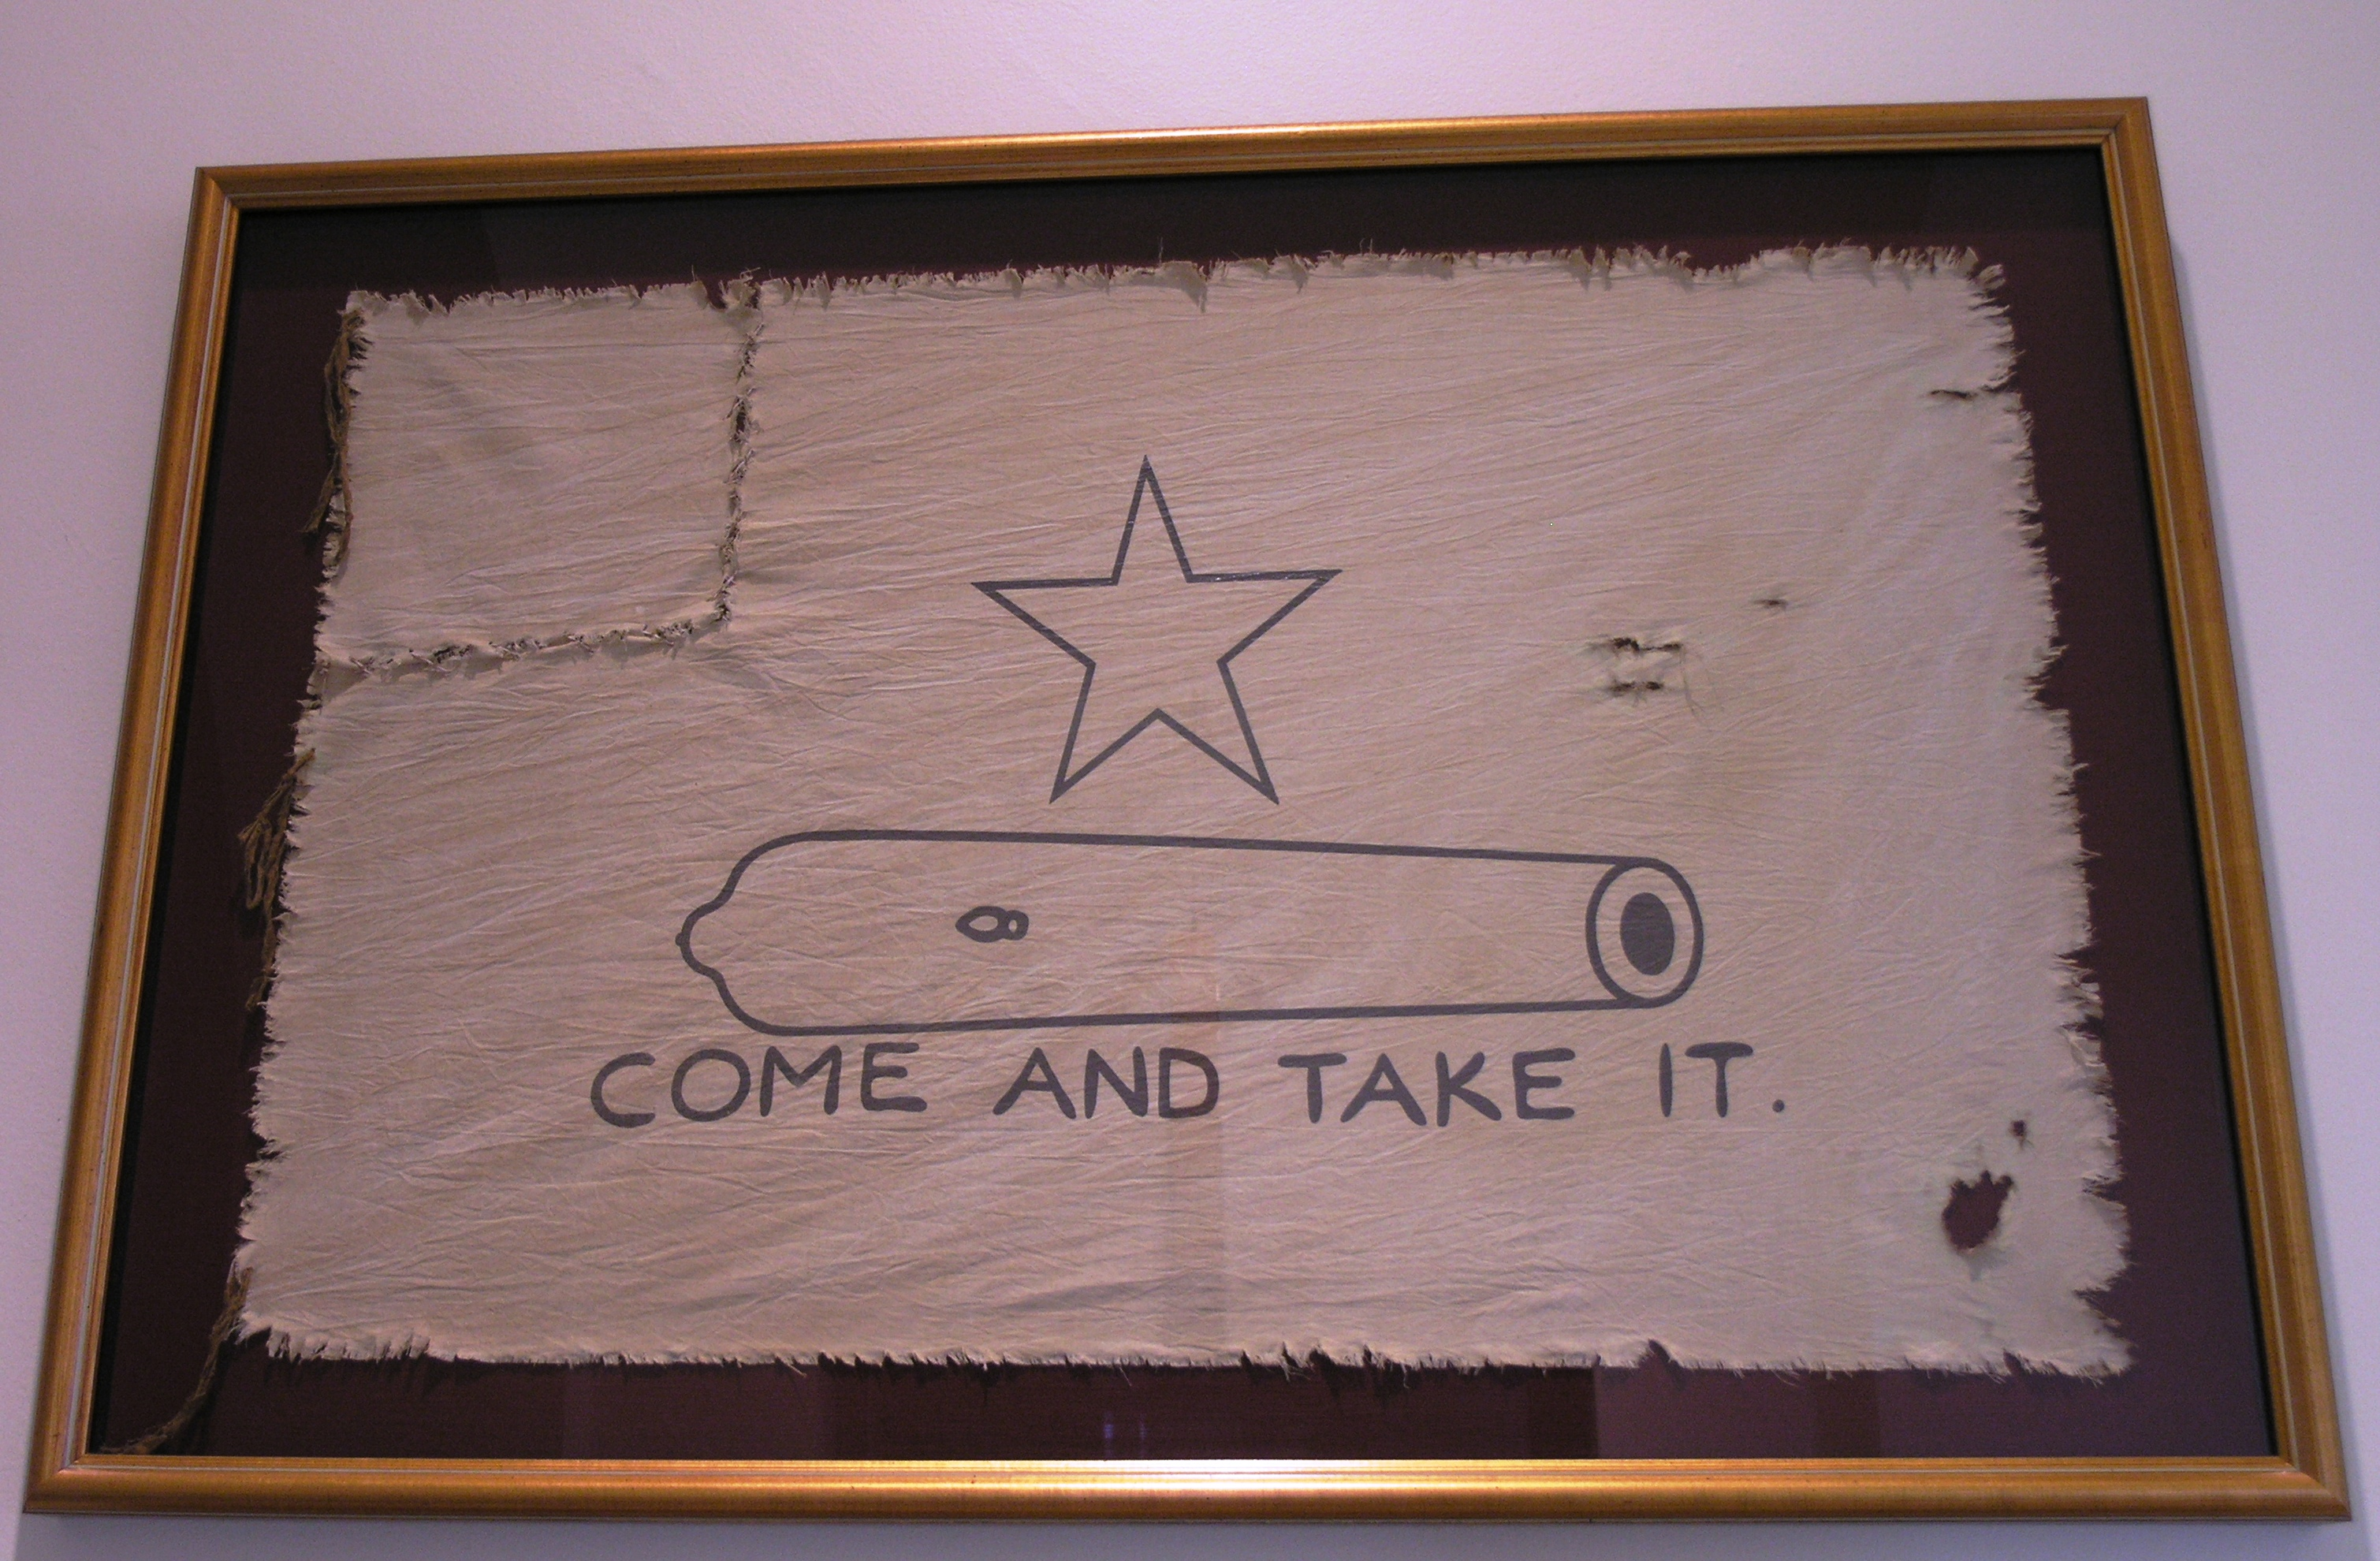
\includegraphics[width=.9\textwidth]{figures/comeAndTakeIt.jpg}
\end{center}
\note{
Those of you -- rightly or wrongly -- involved in the teaparty or in defending gun rights probably recognize this flag with the star and canon on it and with the motto `Come and Take It'.  This flag has been co-opted by those groups to represent resistance against the over-reach of big government.  But, when a Texan, like myself sees this flag, we feel a special connection.  We `know' what it is, and we `know' where it comes from.  This flag, which hangs in the Texas state capitol building, is a replica of the original flag that hung over the town of Gonzales, Texas.  It marks the beginning of the Texas revolution against Mexico.  The actual swivel cannon was mounted to a blockhouse in Gonzales, Texas. A small group of Texians successfully resisted the Mexican forces who had orders from Col. Domingo de Ugartechea to seize their cannon.  The star on this flag is the same star that's present in the Texas flag.  That star has nothing to do with the United States.  It has everything to do with the independence of Texans.
}
\end{frame}
